\documentclass[12pt]{article}
\usepackage[utf8]{inputenc}
\usepackage{amsmath}
\usepackage[margin=1in]{geometry}
\usepackage{tikz}
\usetikzlibrary{positioning}
\usepackage{blindtext}
\usepackage{graphicx}
\usepackage{float}
\usepackage[hidelinks]{hyperref}

\title{Week 9 Notes}
\author{Dylan Ang}
\date{May 2021}

\begin{document}

\maketitle

\tableofcontents

% ========== ========== ========== ==========

\section{Biogeochemistry}

\subsection{Carbon}

\subsubsection{The Global Carbon Cycle}

% \begin{figure}[H]
%     \centering
%     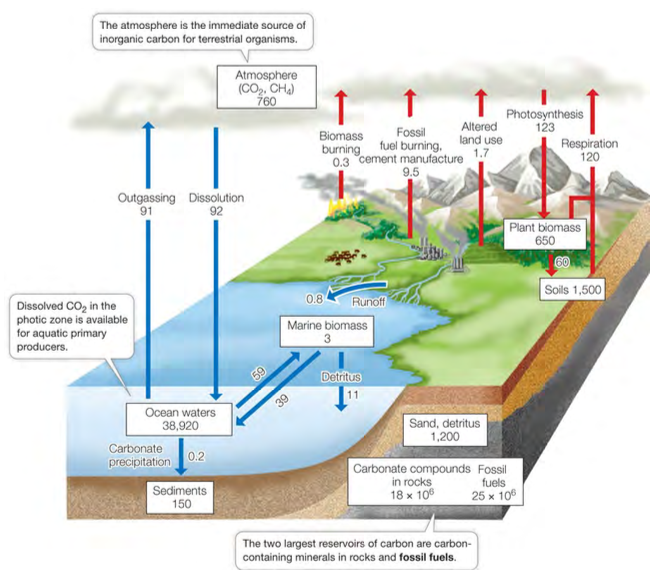
\includegraphics[width=5in]{global-carbon-cycle.png}
%     \caption{The Global Carbon Cycle}
%     \label{global-carbon-cycle}
% \end{figure}

\paragraph{The Global Carbon Cycle: Figure \ref{global-carbon}}
\begin{itemize}
    \item Boxes represent carbon pools
          \begin{itemize}
              \item A carbon pool is a specific area in the ecosystem where carbon can exist.
              \item Pools with a higher number store more carbon mass, the largest being Rock Components and Fossil Fuels. However, there are no arrows coming off of these, so the largest pool that is active is Ocean Waters.
          \end{itemize}
    \item Arrows represent Fluxes.
          \begin{itemize}
              \item Fluxes represent processes that cause movement of carbon from one pool to another.
              \item Fluxes with a higher number transfer more carbon mass. The largest being photosynthesis.
          \end{itemize}
\end{itemize}

\begin{figure}[H]
    \centering
    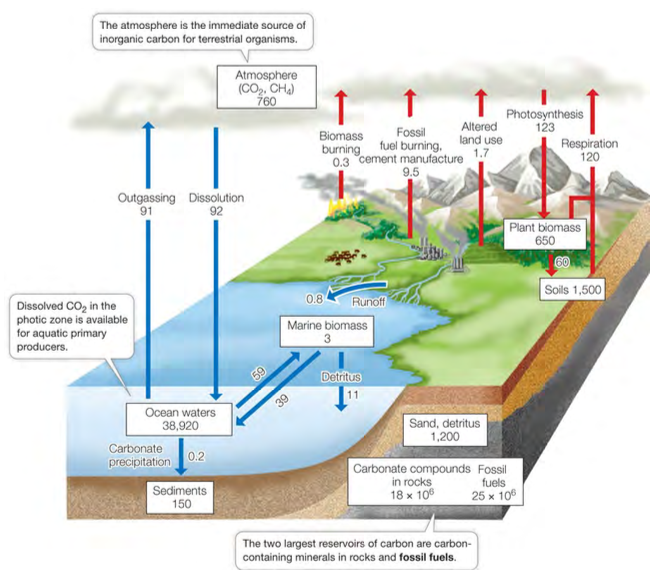
\includegraphics[width=5in]{global-carbon-cycle.png}
    \caption{The Global Carbon Cycle}
    \label{global-carbon}
\end{figure}

\subsubsection[Atmospheric Carbon Dioxide Levels]{Atmospheric $CO_2$ Levels}

\begin{figure}[tph]
    \centering
    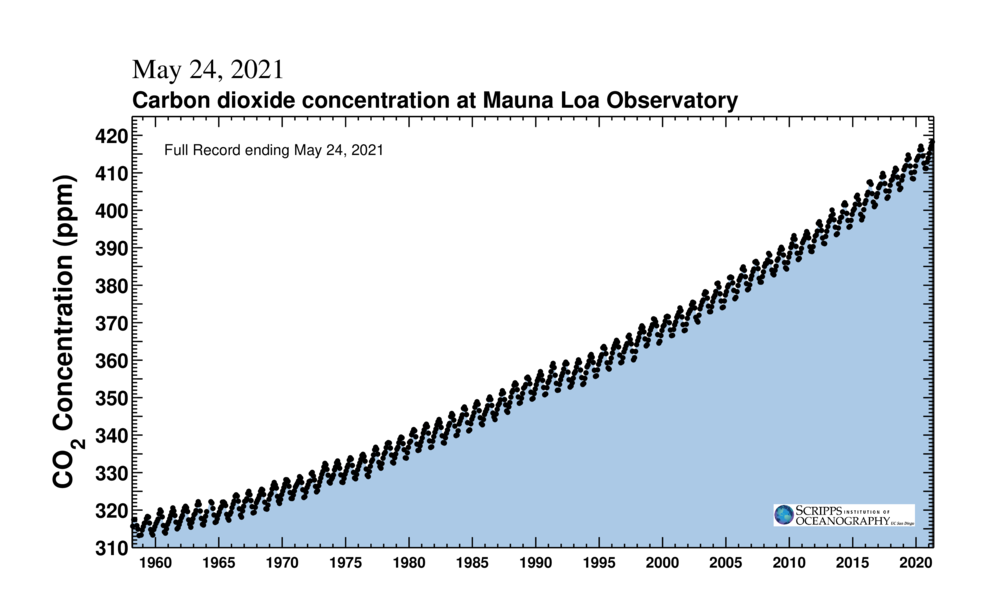
\includegraphics[width=5in]{keeling-curve.png}
    \caption{The Keeling Curve}
    \label{keeling-curve}
\end{figure}

\paragraph{Questions: in Figure \ref{keeling-curve}}
\begin{itemize}
    \item What process drives the overall increase in $CO_2$ levels?
          \begin{itemize}
              \item Anthropogenic greenhouse emissions: fossil fuels.
          \end{itemize}
    \item What process drives the annual oscillation in $CO_2$ levels?
          \begin{itemize}
              \item Global photosynthesis absorbs more $CO_2$ than Respiration creates when plants are growing, i.e., May to September.
              \item Global photosynthesis absorbs less $CO_2$ than Respiration creates when plants are not growing.
          \end{itemize}
    \item Highly seasonal, highly productive ecosystems like boreal forests will experience the most oscillation of $CO_2$ levels, because the carbon they absorb in Spring and Summer is not offset enough by the Southern hemisphere's Fall and Winter.
          \begin{itemize}
              \item Global $CO_2$ level oscillations are mainly driven by the boreal forest.
              \item Locations such as Mauna Loa or the South Pole will also see oscillations, although these are actually residual effects of the boreal forest.
              \item Locations that are not highly seasonal or highly productive will not be able to contribute to global $CO_2$ level oscillations.
          \end{itemize}
\end{itemize}

\paragraph{Ocean Acidification Example}
\begin{itemize}
    \item Higher Acidity (lower pH) and warming of ocean bleaches coral.
    \item Coral have an mutualistic relationship with zooxanthellae.
          \begin{itemize}
              \item Coral get sugar from photosynthesis of zooxanthellae.
              \item Zooxanthellae gets place to live, and nutrients from coral.
              \item Also obligate relationship for coral. Coral can not survive without the relationship.
          \end{itemize}
    \item Higher acidity or warming of the ocean acts as a stressor, killing zooxanthellae.
    \item Without the presence of zooxanthellae, the coral will lose its color (Coral Bleaching) and eventually die if prolonged. If conditions improve after bleaching but before death, the coral can recover by recruiting new zooxanthellae.
\end{itemize}

\subsection{Water and Nitrogen}

\subsubsection{The Global Hydrological Cycle}

\begin{figure}[tph]
    \centering
    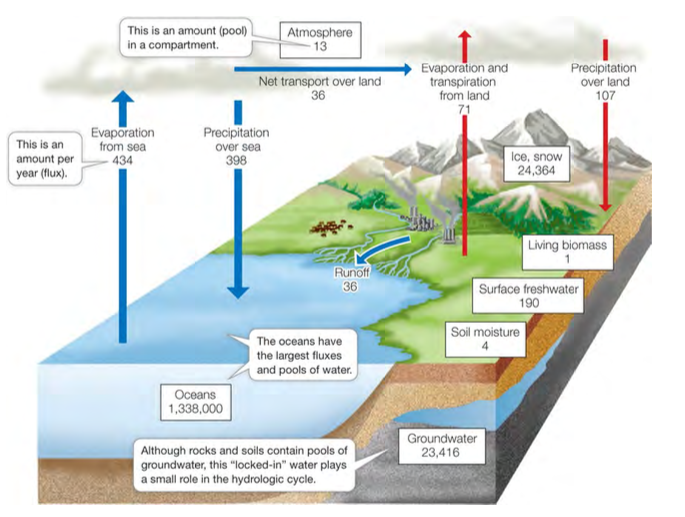
\includegraphics[width=5in]{global-hydrological-cycle.png}
    \caption{The Global Hydrological Cycle}
    \label{global-hydrological}
\end{figure}

\paragraph{The Global Hydrological Cycle: Figure \ref{global-hydrological}}
\begin{itemize}
    \item Fluxes are processes by which water moves from one pool to another.
          \begin{itemize}
              \item Evaporation
              \item Transpiration
              \item Rain
          \end{itemize}
    \item Pools are locations that store water.
          \begin{itemize}
              \item Oceans
              \item Lakes
              \item Groundwater
          \end{itemize}
    \item Largest
          \begin{itemize}
              \item Flux: Evaporation from oceans
              \item Pool: Oceans
          \end{itemize}
    \item Anthropogenic Fluxes
          \begin{itemize}
              \item Groundwater does not naturally connect to the rest of the hydrological cycle.
              \item Humans can, through irrigation and aquifers, access groundwater and thus connect it to the cycle.
          \end{itemize}
\end{itemize}

\begin{figure}[tph]
    \centering
    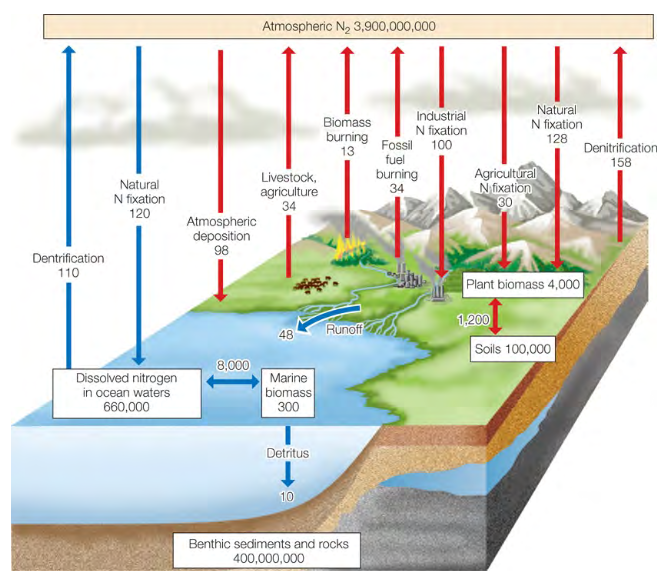
\includegraphics[width=5in]{global-nitrogen-cycle.png}
    \caption{The Global Nitrogen Cycle}
    \label{global-nitrogen}
\end{figure}

\paragraph{The Global Nitrogen Cycle: Figure \ref{global-nitrogen}}
\begin{itemize}
    \item Largest
          \begin{itemize}
              \item Flux: Denitrification - gaseous loss of nitrogen from the soil converting into $N_2$ gas in the atmosphere.
              \item Pool: Atmospheric $N_2$
          \end{itemize}
    \item Anthropogenic fluxes
          \begin{itemize}
              \item Agricultural/Industrial Nitrogen fixation
              \item Fossil fuels, biomass burning, livestock
          \end{itemize}
\end{itemize}

\subsection{Linking Cycles}

\subsubsection{Runoff}

\begin{itemize}
    \item Runoff as a flux: being dissolved in water adds that compound to the water cycle, helping to move it around. All 3 cycles experience runoff.
    \item  Watersheds: Patterns of runoff across land.
\end{itemize}

\paragraph{The gulf of Mexico Dead Zone}
\begin{itemize}
    \item Cause
          \begin{itemize}
              \item Large portion of the Midwest is one watershed, runs off into the Gulf of Mexico.
              \item Chemical runoff: Municipal waste (poo), fertilizer (also poo)
              \item Nitrogen is often a limiting resource, so the nitrogen runoff from fertilizer and other poo causes an algal bloom.
              \item When the algae die, the decomposition of their bodies uses all of the oxygen in the water column.
              \item Low oxygen levels in water column along the coast of the Gulf of Mexico.
          \end{itemize}
    \item Reducing the Dead Zone
          \begin{itemize}
              \item Hurricanes/windstorms mix up water and infuse oxygen.
          \end{itemize}
    \item Impacts of Dead Zone
          \begin{itemize}
              \item Female fish in hypoxic locations have lower fecundity/smaller ovaries.
              \item Male fish have smaller testes and lower sperm production.
          \end{itemize}
\end{itemize}

\subsubsection{How the Carbon cycle connects to the Nitrogen Cycle}

\begin{itemize}
    \item Photosynthesis takes $CO_2$ out of the atmosphere and turns it into sugars.
    \item \textit{Rubisco} is the protein that actually picks up the $CO_2$ from the atmosphere.
    \item \textit{Rubisco} is made up of a lot of nitrogen.
    \item Plants require lots of nitrogen to capture $CO_2$.
\end{itemize}

% ========== ========== ========== ==========

\section{Energy and Trophics}

\subsection{Ecosystem Energy}

\subsubsection{Terms}
\begin{itemize}
    \item Gross Primary Production = rate of photosynthesis
    \item Net Primary Production = GPP - rate of respiration
    \item Food chains are usually simplified, they are more linear.
    \item Food webs better represent reality. Each species may have multiple predators and prey.
\end{itemize}

\begin{figure}[tph]
    \centering
    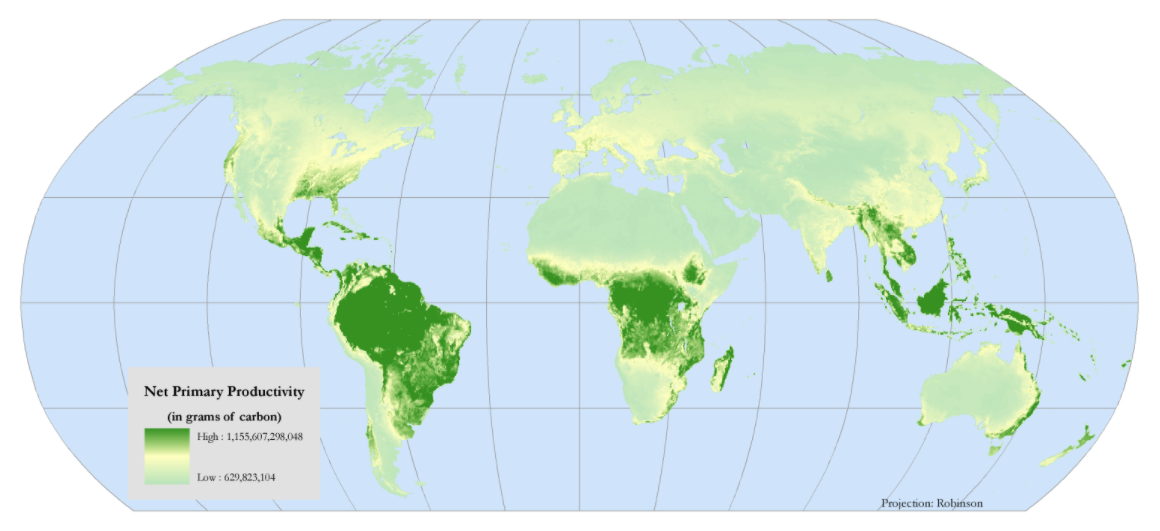
\includegraphics[width=5in]{npp-map.png}
    \caption{Global Net Primary Productivity} \label{npp-map}
\end{figure}

\subsubsection{Trends in NPP maps: Figure \ref{npp-map}}
\begin{itemize}
    \item Higher productivity in tropics. Generally speaking higher temperatures.
    \item Lower productivity in low temperatures and extremely hot temperatures (Sahara)
\end{itemize}

\begin{figure}[tph]
    \centering
    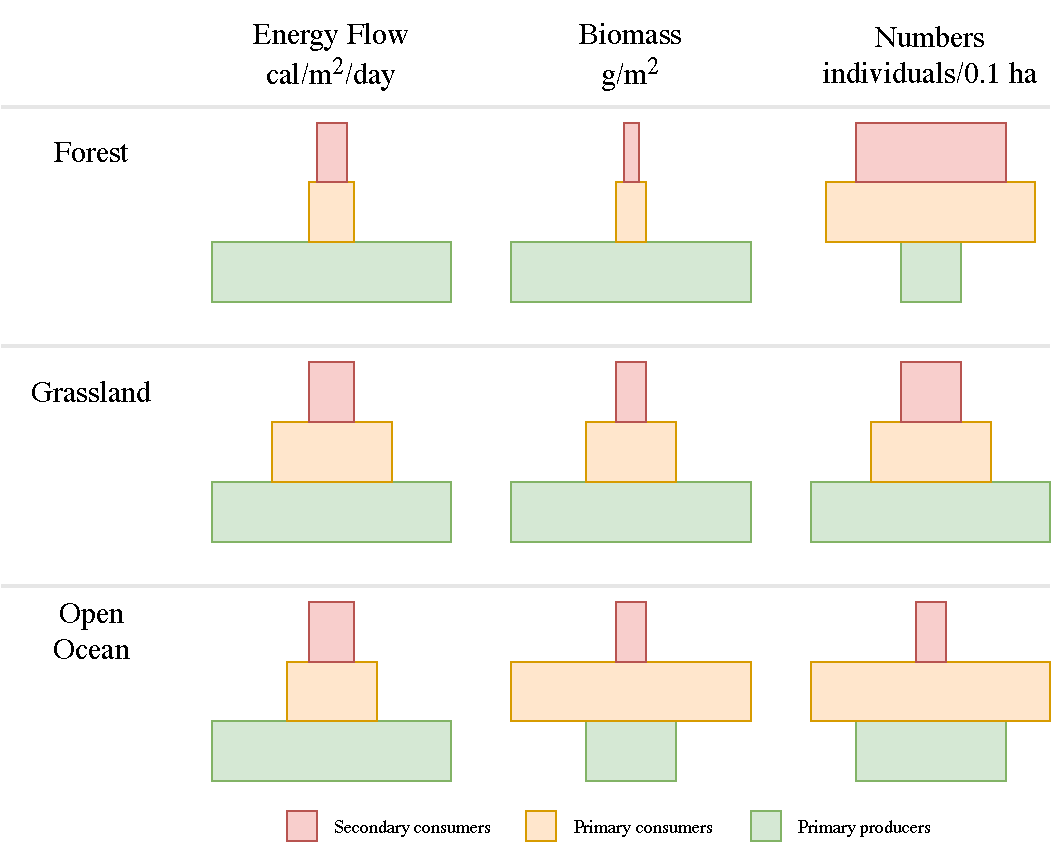
\includegraphics[width=5in]{energy-loss-trophic.pdf}
    \caption{Trophic Pyramids} \label{trophic-pyramids}
\end{figure}

\subsubsection{Trends in Trophic Pyramids: Figure \ref{trophic-pyramids}}
\begin{itemize}
    \item Energy flow is always decreasing from primary producers upwards.
          \begin{itemize}
              \item All energy in the system must come from the producers, and it can only be lost from there.
          \end{itemize}
    \item Why is the biomass decrease more drastic in forests than in grasslands?
          \begin{itemize}
              \item The primary consumers in forests are trees, and the primary consumers in grasslands are grass. Grass is edible by the secondary consumers, but trees are rarely eaten. The secondary consumers are likely only eating the leaves, not the wood (save for termites and decomposers). Therefore the energy that went to growing the wooden trunk and branches will not pass on to the next trophic level.
          \end{itemize}
    \item Explain the difference in numbers between forests and grasslands.
          \begin{itemize}
              \item One tree provides more food than one unit of grass. So, less tree individuals are required to support the primary consumers than grass individuals.
          \end{itemize}
    \item How does the open ocean support more primary consumers than primary producers both in number and biomass?
          \begin{itemize}
              \item The primary producers (mainly algal communities and phytoplankton) have high rates of reproduction. One individual producer can support multiple consumers just through reproducing quickly.
          \end{itemize}
\end{itemize}

\subsubsection{Energy Efficiency and Lindeman's Law}

\begin{figure}[tph]
    \centering
    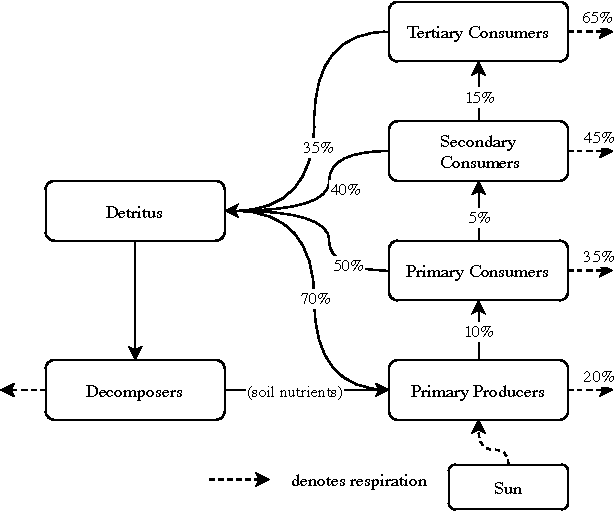
\includegraphics[width=5in]{lindeman.pdf}
    \caption{Lindeman} \label{lindeman}
\end{figure}

\paragraph{In Figure \ref{lindeman}}
\begin{itemize}
    \item On average about 10\% of energy available at one trophic level is transferred to the next trophic level.
    \item Most energy was lost when organisms died.
\end{itemize}

\begin{figure}[tph]
    \centering
    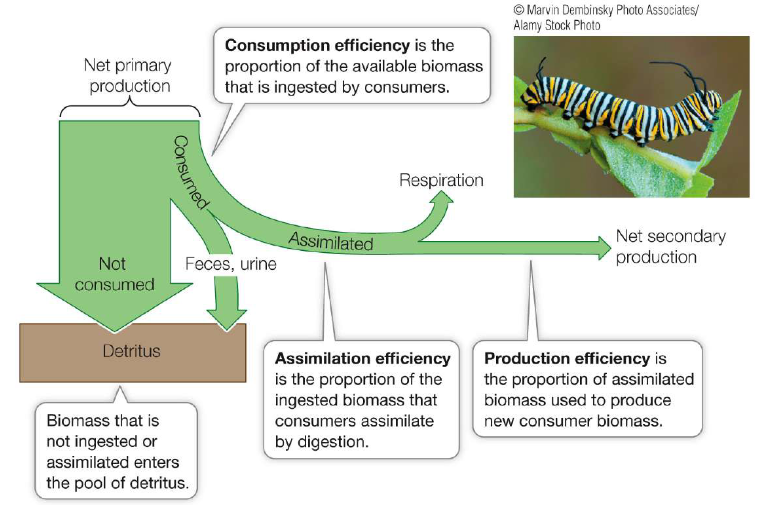
\includegraphics[width=5in]{trophic-sankey.png}
    \caption{Efficiency within a trophic level} \label{trophic-sankey}
\end{figure}

\subsubsection{Efficiency Problems}

\begin{center}
    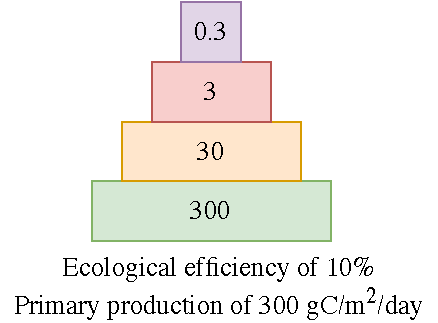
\includegraphics[]{week9-efficiency-problem.pdf}
\end{center}

Notice how primary production is the amount of energy at the lowest trophic level, and each successive level is 10\% of its parent value.

\subsubsection{Determinants of trophic level count}
\begin{itemize}
    \item The number of trophic levels in an ecosystem is limited by
          \begin{itemize}
              \item Available energy (primary productivity)
              \item Efficiency of energy transfer across trophic levels
          \end{itemize}
\end{itemize}

\subsection{Trophic Roles and Interactions}

\subsubsection{Important Role}
\begin{itemize}
    \item Keystone species
          \begin{itemize}
              \item Species that is important for the structure of a given ecosystem. By definition they are not very common within the ecosystem.
          \end{itemize}
    \item Foundation species
          \begin{itemize}
              \item The most common species. They often physically provide a foundation upon which other organisms operate.
          \end{itemize}
    \item Ecosystem engineer species
          \begin{itemize}
              \item Alters the physical structure of the habitat to benefit itself and others.
          \end{itemize}
\end{itemize}

\subsubsection{Examples}

\paragraph{Keystone Species}
\begin{itemize}
    \item Pisaster Starfish
          \begin{itemize}
              \item Removal of Pisaster starfish dramatically reduced diversity.
              \item The Pisaster starfish fed on multiple different species, keeping their populations in check.
              \item Competition increased, top competitor won.
          \end{itemize}
    \item Prairie Dogs
          \begin{itemize}
              \item Prairie dogs serve as prey for higher trophic levels. They burrow holes that provide shelter for other animals, and disturb grazing patterns.
              \item Removal of prairie dogs would have a drastic effect on many different species.
          \end{itemize}
\end{itemize}

\paragraph{Foundation Species}
\begin{itemize}
    \item Corals
          \begin{itemize}
              \item Coral reef provides habitat for many different species.
              \item Without coral, all of the coral reef residing animals must find a new place to live.
          \end{itemize}
    \item trees
          \begin{itemize}
              \item The tree is a habitat for other organisms.
          \end{itemize}
\end{itemize}

\paragraph{Ecosystem Engineers}
\begin{itemize}
    \item Beavers
          \begin{itemize}
              \item Beavers chew down trees and build dams.
              \item Alter the plant community and flow patterns downstream.
              \item Beaver activity leads to higher diversity across the entire ecosystem.
          \end{itemize}
\end{itemize}

\subsubsection{Overlapping Roles}
\begin{itemize}
    \item A single species can not be both a keystone species as well as a foundation species.
          \begin{itemize}
              \item This is because keystone species are by definition, rare and impactful. Whereas foundation species are by definition, frequent and impactful.
          \end{itemize}
\end{itemize}

\subsubsection{Top Down and Bottom Up Effects}

\paragraph{Definition}
\begin{itemize}
    \item Top Down
          \begin{itemize}
              \item Change begins in predator species and the effects trickle down to the trophic levels.
          \end{itemize}
    \item Bottom Up
          \begin{itemize}
              \item Change begins in lower trophic levels and the effects trickle up into higher trophic levels.
          \end{itemize}
\end{itemize}

\paragraph{Examples}
\begin{itemize}
    \item Sea Otter: Top Down
          \begin{itemize}
              \item Sea Otter populations decline $\Rightarrow$ Sea Urchin populations increase $\Rightarrow$ Kelp forest biomass declines.
          \end{itemize}
    \item Algae: Bottom up
          \begin{itemize}
              \item Nutrient rich water $\Rightarrow$ Algal bloom $\Rightarrow$ Less oxygen in water column as algae die $\Rightarrow$ Fish have less oxygen and die out.
          \end{itemize}
\end{itemize}

% ========== ========== ========== ==========

\section{History of Life}

\subsection{Types of Major Events}

\begin{table}[tph]
    \centering
    \begin{tabular}{| l | l |}
        \hline
        Major Geophysical Events          & Major Biological Events                      \\
        \hline
        Tectonics                         & Origin of Life                               \\
        Changes in Earth's magnetic field & Evolution of photosynthesis                  \\
        Atmospheric change                & Evolution of eukaryotes and multicellularity \\
        Changes in Earth's orbit          & The Cambrian Explosion                       \\
        Climate change                    & Colonizing land                              \\
        Sea level change                  & Mass Extinctions                             \\
        Asteroid impacts                  & Major radiations                             \\
                                          & Evolution and migration of humans            \\
        \hline
    \end{tabular}
\end{table}

\subsection{Earth's History in One Giant Graph}

\begin{figure}[tph]
    \centering
    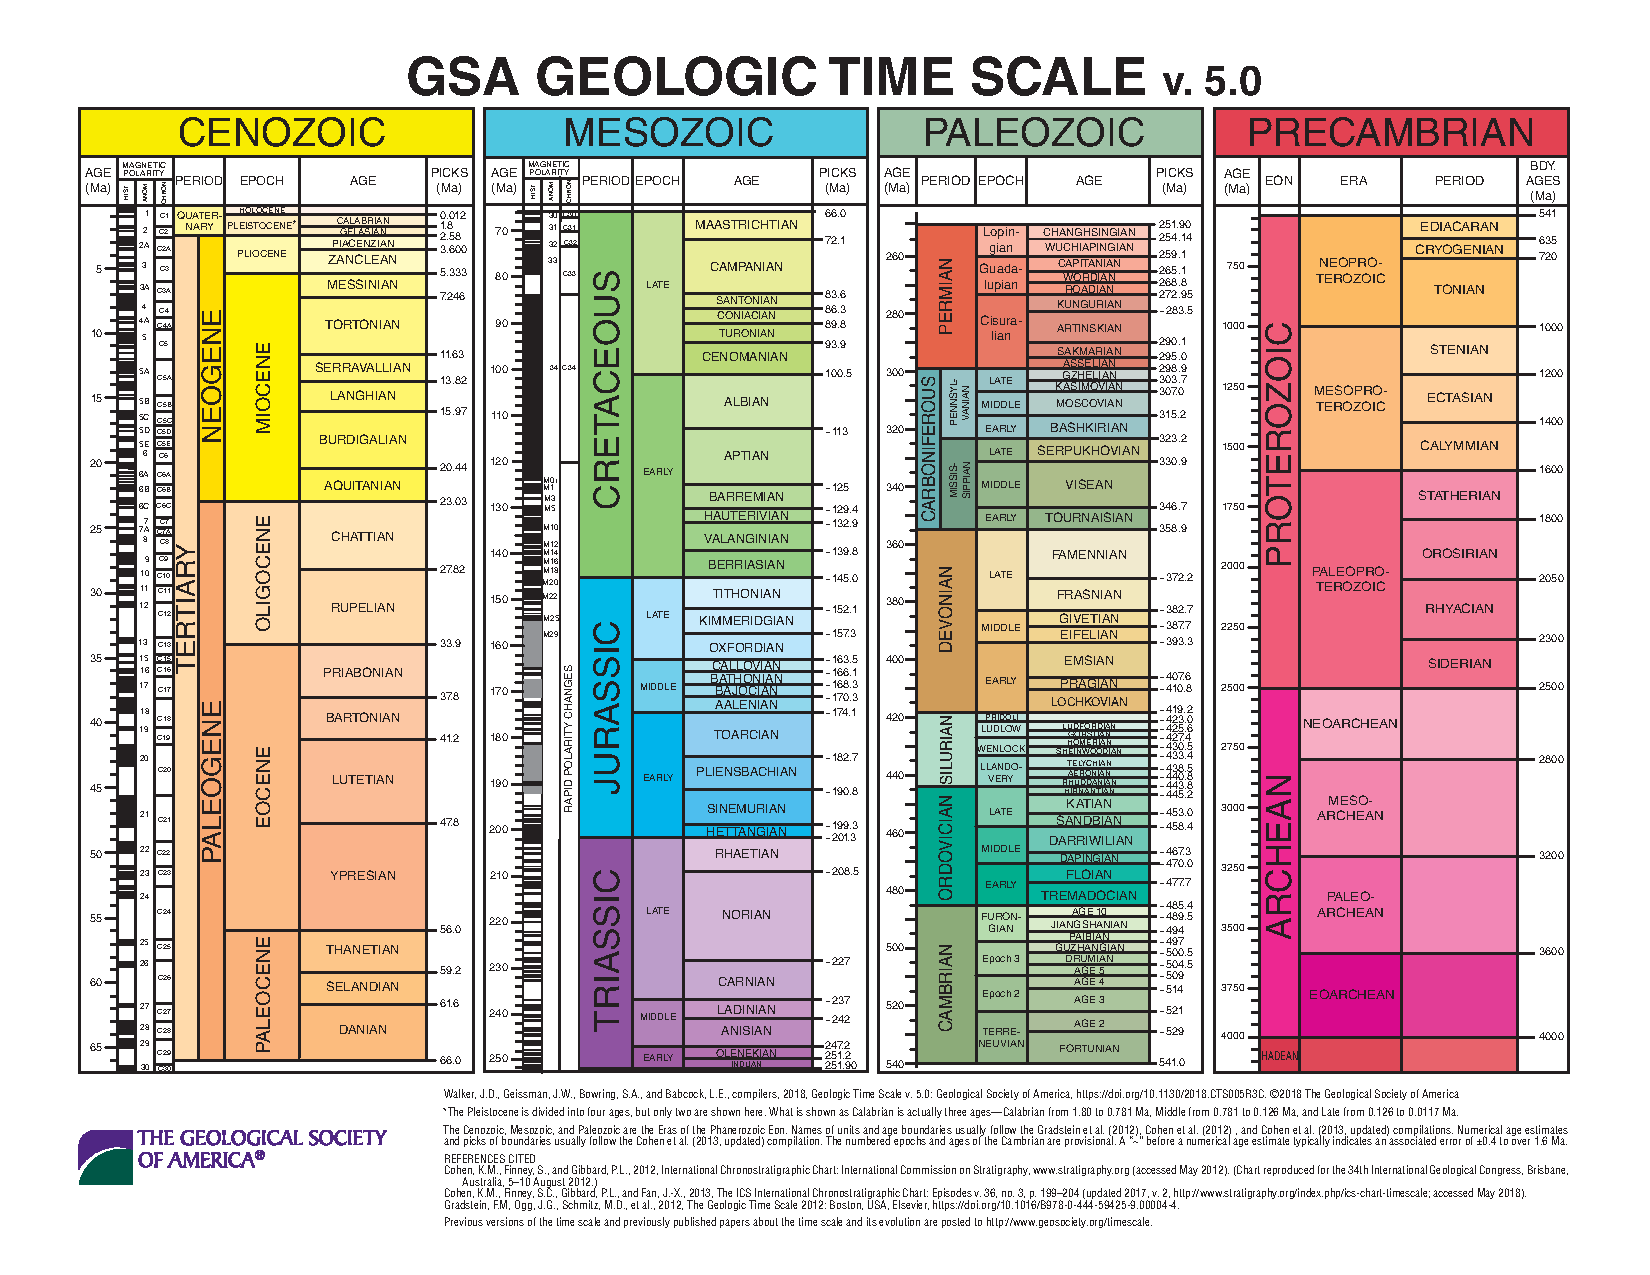
\includegraphics[width=\linewidth]{timescl.pdf}
    \caption{Geological Time Scale} \label{timescl}
\end{figure}

\paragraph{In Figure \ref{timescl}}
The bottom right of the graph represents the beginning of Earth. Chronology is bottom to top, right to left.

\subsection{Origins of Life to the Cambrian Explosion}
\begin{enumerate}
    \item \textbf{Origin of Life (~3.8 bya)} Precambrian/Archean/Eoarchean
          \begin{itemize}
              \item It is believed that life originated 3.8 billion years ago.
              \item Thought to be single celled organisms, bacteria
              \item Lived at the bottom of the ocean in hydrothermal vents, which are places on the ocean floor where super hot, toxic water shoots out at high speed.
              \item These vents are caused by magma near the surface of the ground which boils the water. This water is carrying toxic compounds, metals.
              \item \textit{Chemoautotrophs} in this region use metal compounds and energy from the vents to produce food. They do not rely on sunlight.
          \end{itemize}
    \item \textbf{Photosynthesis (~2.5 bya)} Precambrian, between Neoarchean and Paloproterozoic
          \begin{itemize}
              \item Emergence of $C_3$ photosynthesis
              \item First fossil evidence of life (cyanobacteria).
              \item Production of oxygen $\rightarrow$ allows for aerobic bacteria.
          \end{itemize}
    \item \textbf{Ediacaran period (635-541 mya)} Precambrian/Neoproterozoic
          \begin{itemize}
              \item Animals are mostly flat bodied filter feeders that reside at the bottom of the ocean.
          \end{itemize}
    \item \textbf{The Cambrian Explosion (542-488 mya)} Paleozoic/Cambrian/Epoch 2-3
          \begin{itemize}
              \item Immense diversification of animal life in terms of species and niches.
              \item Evidence of adaptations for predation and defense.
              \item Most of the fossils from this era come from a location in British Columbia, Canada called the Burgess Shale.
              \item Most of the major aquatic animal phyla begin here.
          \end{itemize}
\end{enumerate}

\subsection{Mass Extinctions}

\begin{center}
    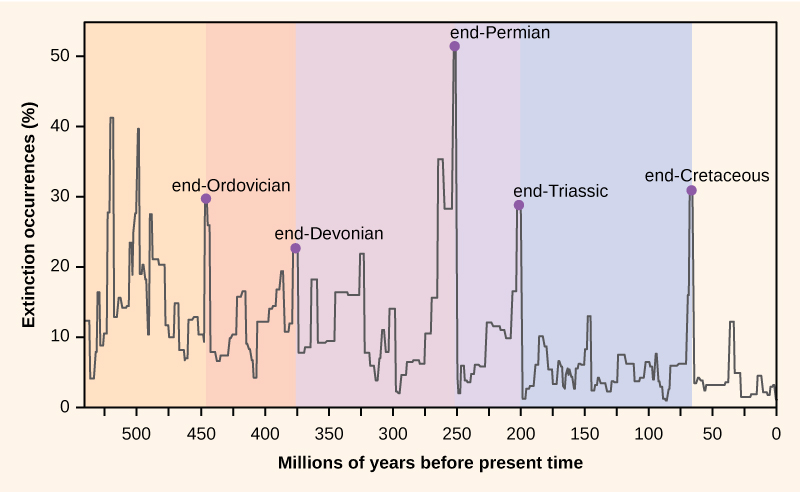
\includegraphics[width=\linewidth]{mass-extinction.jpeg}
\end{center}

\paragraph{Causes}
\begin{itemize}
    \item \textbf{Ordovician (444 mya):} global warming, anoxia, sea level rise?
    \item \textbf{Devonian (359 mya):} asteroid, reduced speciation?
    \item \textbf{Permian (252 mya):} volcanoes, glaciation, sea level drop?
    \item \textbf{Triassic (201 mya):} volcanic release of methane
    \item \textbf{Cretaceous (65 mya):} asteroid impact in Yucatan
    \item \textbf{Holocene (present):} humans
\end{itemize}

\paragraph{After Extinction}
\begin{itemize}
    \item \textbf{Silurian Period (444-419 mya):}
          \begin{itemize}
              \item Origin of land plants
              \item Origin of terrestrial fungi? (mycorrhizae)
              \item Origin of terrestrial arthropods
          \end{itemize}
    \item \textbf{Devonian Period (419-359 mya):}
          \begin{itemize}
              \item The stem tetrapods: transitional fossils in the shift from fish to terrestrial tetrapod groups (amphibians, reptiles, mammals).
              \item Eusthenopteron (fish) $\Rightarrow$ Tiktaalik (transitional) $\Rightarrow$ Icthyostega (tetrapod)
          \end{itemize}
    \item \textbf{Carboniferous Period (359-304 mya):}
          \begin{itemize}
              \item Massive forests, enormous plant diversity
              \item Invasion of land by plants and tetrapods increases level of oxygen to the highest in Earth's history.
              \item Giant insects due to high oxygen.
          \end{itemize}
    \item \textbf{End Permian Mass Extinction (252 mya):}
          \begin{itemize}
              \item Largest mass extinction
              \item Large forests die out $\Rightarrow$ oxygen level drops
              \item Plant life dies, sinks to bottom of ocean/lakes, the pressure of sediments and water compresses this organic matter into oil and coal deposits.
              \item Formation of Pangea
          \end{itemize}
\end{itemize}

\subsection{Dinosaurs to Modern Times}

\begin{itemize}
    \item \textbf{Triassic Period (252-201 mya):}
          \begin{itemize}
              \item First Dinosaurs
              \item First Mammals: mostly small and rodent-like
          \end{itemize}
    \item \textbf{Jurassic Period (201-145 mya):}
          \begin{itemize}
              \item Stegosaurus and Archaeopteryx
          \end{itemize}
    \item \textbf{Cretaceous Period (145-65 mya):}
          \begin{itemize}
              \item Tyrannosaurus rex, Triceratops, Velociraptor
          \end{itemize}
    \item \textbf{End Cretaceous Mass Extinction (65 mya):}
          \begin{itemize}
              \item Thick iridium (rare on earth, common in asteroids) layer at a particular age in the geological strata, which is good evidence of an asteroid impact.
              \item The Chicxulub crater left behind by the asteroid.
          \end{itemize}
    \item \textbf{Early Paleogene Period (~65 mya):}
    \begin{itemize}
        \item Mammals survive the End Cretaceous
        \item 130 new mammal genera arise in about 10 mya
        \item Radiation of Angiosperms (flowering plants)
        \begin{itemize}
            \item Angiosperms perform evapotranspiration (water enters through the plant and exits through the leaves). As Angiosperms evopotranspirate, they alter the hydrologic cycle by adding water into the atmosphere.
            \item They bring the oxygen level back up after the End Permian mass extinction.
            \item Only fruit to produce nectar and fruit $\Rightarrow$ new animal niches
            \item Radiation in Angiosperms caused by specialization into new methods of attracting pollinators.
        \end{itemize}
    \end{itemize}
    \item \textbf{Oligocene Epoch (34-23 mya):}
    \begin{itemize}
        \item Expansion of grasslands and emergence of $C_4$ photosynthesis
        \item Drives the presence of large herbivores that rely on grass diets
    \end{itemize}
    \item \textbf{Prelude to the Pleistocene:}
    \begin{itemize}
        \item Looks like modern life.
        \item Climate comes into the life experience.
    \end{itemize}
\end{itemize}

\subsection{Life History Discussion}



\begin{itemize}
    \item Why do aerobic organisms arise after photosynthesis? How did pre-photosynthesis organisms perform respiration?
    \begin{itemize}
        \item Aerobic respiration is very energy-efficient, but it requires oxygen. So when photosynthesis begins happening, there is a push towards aerobic respiration.
        \item Pre-photosynthesis organisms performed either anaerobic respiration or fermentation.
    \end{itemize}
    \item How did the first organisms get energy without photosynthesis?
    \begin{itemize}
        \item Organisms at this time are Chemoautotrophs, gathering energy from chemical compounds in deep ocean vents.
    \end{itemize}
    \item Why do we see an increase in $O_2$ levels following the invasion of land? What was the terrestrial landscape like at this time?
    \begin{itemize}
        \item Photosynthetic plants invaded land, and the cycad forests begin to really develop and spread quickly.
        \item This increases the oxygen level, supporting large insects.
    \end{itemize}
    \item Why do $O_2$ levels drop so significantly ~250 mya? Why do we not see similar drops at 444, 359, 201, or 65 mya? 
    \begin{itemize}
        \item At this time, 90\% of life dies out, including the cycad forests that raised the oxygen to such high levels in the first place. Therefore there is a large drop in the oxygen as the forests no longer photosynthesize.
        \item At this time, there is a major rise in plant growth, followed by a mass extinction event. This is unique to the Permian. 
    \end{itemize}
    \item The largest increase in genera is seen in the recent past, why then is the Cambrian Period considered an explosion of life?
    \begin{itemize}
        \item The Cambrian saw the very first explosion of life.
        \item Very important basic changes that set the stage for the future such as many of the genera we see today, as well as resource strategy niches like predation.
    \end{itemize}
    \item What is the overall pattern? What does this indicate about the resilience of life on Earth?
    \begin{itemize}
        \item Appears to fit an exponential growth curve. 
        \item Even when mass extinction events happen, something will survive.
        \item Surviving organisms have reduced competition and radiate quickly.
    \end{itemize}
\end{itemize}

\end{document}